% الجزء: sets-functions-relations
% الفصل: relations
% القسم: trees

\documentclass[../../../include/open-logic-section]{subfiles}

\begin{document}

\olfileid[ar]{sfr}{rel}{tre}
\olsection{الأشجار}

من الأنواع الخاصة للترتيب الجزئي التي تؤدي دورًا مهمًا في جميع فروع
المنطق \emph{الشجرة}. وتظهر الأشجار المنتهية في الأجزاء الأولية من المنطق؛
فيمكن، مثلًا، فهم !!{formula}s من حيث تحليلها إلى شجرة تركيبية، كما تتخذ
!!{derivation}s في كثير من أنساق !!{derivation} أيضًا صورة أشجار منتهية.
%
أما الأشجار غير المنتهية فتظهر بالفعل في براهين مبرهنات الاكتمال للمنطق القضي
ومنطق الرتبة الأولى، وتستعمل في المنطق الرياضي كله.

يرتبط مفهوم الشجرة في نظرية المجموعات ارتباطًا وثيقًا بفكرة الشجرة في
نظرية الرسوم البيانية. وفيما يلي صورة لشجرة (منتهية):

\begin{center}
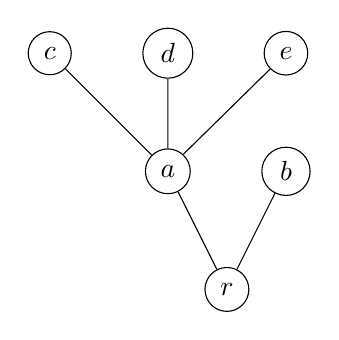
\begin{tikzpicture}[nodes={draw, circle}, -]
\node{$r$} [grow'=up]
    child { node {$a$} 
        child { node {$c$} }
        child { node {$d$} }
        child { node {$e$} }
    }
    child { node {$b$} };
\end{tikzpicture}
\end{center}

العقدة السفلى~$r$ هي الجذر. ولكل عقدة غير $r$ عقدة أصل واحدة بالضبط تقع
تحتها مباشرة. ويمكننا أن نعد العلاقة التي تقوم بين عقدة~$x$ وعقدة~$y$،
حين يمكن بلوغ $y$ من~$x$ بتتبع الحواف إلى أعلى، هي كون $x$
\emph{سلفًا} لـ~$y$.

علاقة السلف في الشجرة ترتيب جزئي صارم. وهذا يحفز التعريف بالمجموعات.
ولصياغته نحتاج إلى مفهومين. يكون \emph{العنصر الأصغر} في مجموعة~$A$
مرتبة جزئيًا بـ~$\le$ هو !!a{element} $x \in A$ بحيث يصدق، لكل
$y \in A$، أن~$x \le y$. وتكون المجموعة \emph{مرتبة ترتيبًا جيدًا}
بـ~$\le$ إذا كان لكل مجموعة جزئية غير خالية منها عنصر أصغر.

\begin{defn}[الشجرة]
\emph{الشجرة} هي زوج $T = \tuple{A, \le}$ بحيث تكون $A$ مجموعة، وتكون
$\le$ ترتيبًا جزئيًا على~$A$ له عنصر أصغر وحيد $r \in A$ (يسمى
\emph{الجذر})، ولكل $x \in A$، تكون المجموعة $\Setabs{y}{y \le x}$
مرتبة ترتيبًا جيدًا بـ~$\le$.
\end{defn}

\begin{defn}[اللواحق]
لتكن $T = \tuple{A, \le}$ شجرة.
إذا كان $x,y \in A$ وكان $x < y$، ولم يوجد $z \in A$ بحيث
$x < z < y$، قلنا إن $y$ \emph{لاحق} لـ~$x$.
\end{defn}

تسمى لواحق $x \in A$ أيضًا \emph{أبناءه}. وإذا كان
$y$ لاحقًا لـ~$x$، سمينا $x$ \emph{السابق} لـ~$y$ أو
\emph{العقدة الأصل} لها.

\begin{prop}
إذا كان $\tuple{A,\le}$ شجرة، فإن لكل $x \in A$ غير الجذر سابقًا واحدًا
على الأكثر.
\end{prop}

\begin{proof}
  افترض أن $y_1 < x$ و$y_2 < x$ وأن $y_1 \neq y_2$. عندئذ
  $\{y_1, y_2\} \subseteq \Setabs{z}{z<x}$. وبما أن
  $\Setabs{z}{z<x}$ مرتبة ترتيبًا جيدًا بـ~$\le$، فإن لمجموعتها الجزئية
  $\{y_1, y_2\}$ عنصرًا أصغر، ولا بد بداهةً أن يكون إما $y_1$ أو~$y_2$.
  ومن ثم فإما أن $y_1 \le y_2$ أو أن $y_2 \le y_1$. وقد افترضنا أن
  $y_1 \neq y_2$، ولذلك فإما أن $y_1 < y_2$ أو أن $y_2 < y_1$. وبما
  أننا افترضنا أيضًا أن $y_1 < x$ و$y_2 < x$، يكون إما
  $y_1 < y_2 < x$ أو $y_2 < y_1 < x$. ومن ثم لا يمكن أن يكون كل من
  $y_1$ و$y_2$ سابقًا لـ~$x$.
\end{proof}

\begin{defn}
يقال إن الشجرة $T = \tuple{A, \le}$ \emph{غير منتهية} إذا كانت $A$
مجموعة غير منتهية، وإنها \emph{منتهية} في غير ذلك. وإذا كانت $T$ بحيث
يكون لكل $x \in A$ عددًا منتهيًا فقط من اللواحق، قلنا إن $T$
\emph{منتهية التفرع}.
\end{defn}

\begin{defn}[الفروع]
إذا أعطيت شجرة $T = \tuple{A, \le}$، كان \emph{الفرع} من~$T$ سلسلة
قصوى في~$T$، أي مجموعة $B \subseteq A$ بحيث يكون، لأي $x, y \in B$،
واحد على الأقل من $x \le y$ و$y \le x$ صادقًا، ولكل
$z \in X \setminus B$ يوجد $u \in B$ بحيث لا $z \le u$ ولا $u \le z$.
%
ونستعمل $[T]$ للدلالة على مجموعة جميع فروع $T$.
\end{defn}

\begin{ex}
من الأمثلة التقليدية على الأشجار المنتهية التفرع \emph{الشجرة الثنائية
غير المنتهية} للمتتاليات المنتهية من الرمزين $0$ و~$1$، ويرمز إليها
أحيانًا بـ$\{0,1\}^*$ أو~$\Bin^*$، وتُرتب بعلاقة الامتداد $\sqsubseteq$
(مثلًا، $101 \sqsubseteq 101101$). وبما أنه يمكن دائمًا تمديد أي سلسلة
ثنائية بإضافة $0$ أو $1$ إلى نهايتها، فإن هذه الشجرة تحوي عددًا غير
منته من العناصر: فلكل عنصر~$s$ لاحقان بالضبط، هما $s0$ و~$s1$. وجذرها
هو المتتالية الخالية $\emptyseq$.
\end{ex}

\begin{ex}
وبصورة أعم قليلًا، فإن مجموعة المتتاليات المنتهية من الأعداد
الطبيعية~$\Nat^*$ مع علاقة الامتداد~$\sqsubseteq$ شجرة أيضًا. ومن الواضح
أنها ليست منتهية التفرع: فلكل $s \in \Nat^*$ عدد غير منته من اللواحق~$sn$،
واحد لكل $n \in \Nat$. وكل مجموعة $A \subseteq \Nat^*$ مغلقة
تحت~$\sqsubseteq$ هي \emph{شجرة جزئية} من~$\Nat^*$. (أي إن $A$ تكون بحيث
إذا كان $s \in A$ وكان $s' \sqsubseteq s$، فإن $s' \in A$ أيضًا.) ويمكن
تمثيل جميع الأشجار المنتهية بأشجار جزئية منتهية من~$\Nat^*$.
\end{ex}

\begin{prop}[قضية \foreignlanguage{english}{K\H{o}nig} المساعدة]
إذا كانت $T = \tuple{A,\le}$ شجرة غير منتهية ومنتهية التفرع، فإن لـ$T$
فرعًا غير منته.
\end{prop}

ومن الحالات الخاصة لقضية \foreignlanguage{english}{K\H{o}nig} المساعدة، الواسعة الاستعمال في نظرية
قابلية الحساب، ما يعرف باسم \emph{الصيغة الضعيفة من قضية \foreignlanguage{english}{K\H{o}nig} المساعدة}، وهي الآتية:
لكل شجرة جزئية غير منتهية من $\{0,1\}^*$ فرع غير منته.

\end{document}
